\section{Prospective finance and completed payments}
\label{sec:finance}
\subsection{When the first menu is insufficient}
Across 188 liquidation episodes, agents pay 128 debts and are eliminated in sixty. The complete classification is 128 payments, 56 debts above the generous asset bound, one menu-restricted elimination and three demonstrated-payable bankruptcies. Actual payments plus the three historical payment witnesses yield 131 demonstrated-payable episodes, of which 128 are paid, or 97.7\%. This conditional rate concerns the immediate obligation, rather than whether earlier investment decisions were prudent.

The census contains substantial variation in required execution. Sixty-seven successful payments take one action. Sixty-two can be covered by entry cash and initially listed mortgages, without selling development. A further 52 successful payments can be covered after adding all building salvage without requiring an unlisted mortgage. These categories explain why a high payment rate alone gives little calibration of planning difficulty. Repeated local success remains an observation, but it should not be mistaken for superiority to a simple policy whose performance has not been measured.

Sixteen episodes satisfy the necessary-collateral inequality. In fourteen, agents sell buildings, use mortgages that were absent from the first menu, and pay. In two, they declare bankruptcy at the first decision. The successful texts state the subsequent mortgages or an aggregate budget encompassing them in thirteen episodes. The remaining text, Opus at G20 d291, asks whether clearing the pink houses and mortgaging those deeds could close the gap. We preserve that tentative statement rather than treating it as a completed calculation.

The prospective channels matter. Nine successful statements are applied private notes. Five are provider-returned explanations from Opus recovery responses, which contain no applied note. Across these channels, the initial response often specifies what selling will make possible before that option appears in a refreshed menu. G2 Sol explicitly budgets the yellow mortgages; G5 Gemini corrects an initial shortfall account within its first response and includes both dark-blue mortgages; G18 Gemini identifies the one-house sale that releases Park Place. Full selected first-decision fields for all sixteen episodes accompany the numerical rows in Appendix~\ref{app:finance}.

By configuration, the necessary subset contains payments in 2/3 Sol, 5/6 Gemini, 5/5 Opus and 2/2 Grok episodes. These are unequal encountered positions, not a model ranking. The same systems that fail also succeed elsewhere. The two failures reveal a local omission rather than a demonstrated general boundary of their planning ability.

\begin{figure}[t]\centering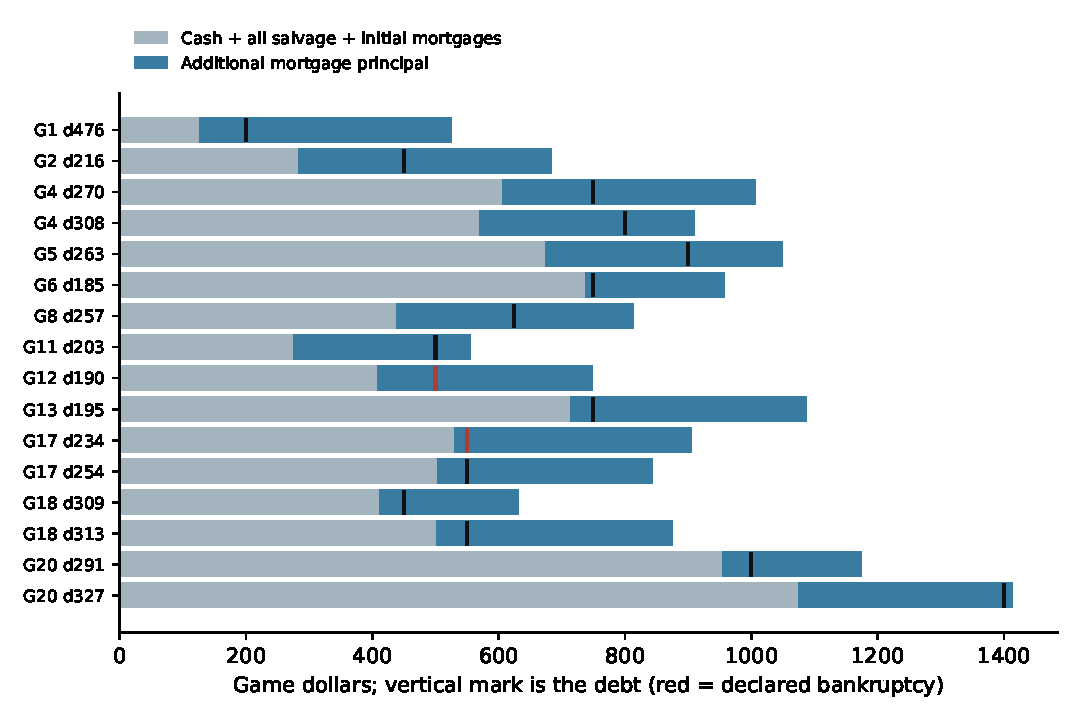
\includegraphics[width=\linewidth]{necessary_collateral.pdf}
\caption{All sixteen necessary-collateral episodes. Gray includes cash, all salvage and initially listed mortgages. Blue adds the remaining mortgage principal in the generous bound. Each debt mark exceeds the gray amount. Red marks identify the two immediate declarations; all other episodes pay. The bars describe resources, not an assumption that every liquidation ordering is legal.}\label{fig:necessary}
\end{figure}

At G12 d190, Sol totals \$53 cash, \$225 building salvage and \$130 listed mortgages, concluding that \$408 cannot pay \$500. Selling would also release \$340 red collateral. At G17 d234, Gemini totals \$500 salvage and a \$30 Baltic mortgage against \$550 owed, omitting \$375 dark-blue collateral. Both statements and declarations are internally consistent with incomplete sums. Historical executable witnesses establish legal payment routes. The observations link stated resource inclusion to continuing liquidation, and stated omission to an immediate stop, without identifying which internal computation produced either response.

The necessity subset differs from the broader use count. Nineteen successful episodes use 33 mortgages absent from their initial menus. Fourteen are the necessary successes above. The other five comprise four G3 Gemini episodes and G18 Sol d428, where the generous initial-resource total already covers the debt. Such mortgages can be chosen even when they are not arithmetically necessary. Reporting nineteen as a success denominator would mix a chosen financing route with a required dependency.

\Needspace{20\baselineskip}
\subsection{An announced endpoint survives ten actions}
\TranscriptTitle{payment}{Liquidation reaches the predicted \$14 remainder}
At G20 turn 107 only Gemini and Sol remain. Sol has \$49, nine orange houses and two brown hotels. Gemini's private note evaluates the rival's liquidation capacity before raising Pennsylvania rent to \$1,400:
\TranscriptQuote{g20-d325-creditor-note}
Sol lands there next turn and states its own budget before selling anything:
\TranscriptQuote{g20-d327-plan}
Two building-sale actions raise \$700. Eight mortgages raise \$665. At the final mortgage Sol records:
\TranscriptQuote{g20-d336-last}
The payment events and next state give \$49+\$700+\$665-\$1,400=\$14. The creditor and debtor both state the correct aggregate, although Gemini's \$675 salvage and \$690 mortgage components each differ by \$25 in opposite directions. Accurate totals therefore coexist with inaccurate components. Sol's statement and completed payment are the stronger correspondence evidence.

Ten is the execution length, not ten levels of lookahead. Removing development releases mortgages, while several subsequent choices can be interchangeable. Updated menus supply intermediate feedback throughout. Sol specifies an aggregate budget and broad policy before acting; it does not enumerate an ordered ten-call plan. The successful continuation demonstrates that it sustains this local objective across the recorded actions. No comparison measures whether it preserves the most valuable residual portfolio or chooses an optimal survival strategy.
\TranscriptSource{G20 d325 and d327--336, standard responses. All three fields are private notes and are not claimed to reach another player. Original turn-108 events establish sales, mortgages and payment.}

The third payable bankruptcy illustrates a different separation. G12 Grok's note recognizes that staged pink sales can pay \$250, while content describes a sale and the received call declares bankruptcy. The historical five-sale route leaves \$43. That episode is not in the necessary-collateral subset. It shows why a useful statement cannot substitute for the action that controls play. Successful assessment, channel agreement and successful execution are separate observables even within the same short financial task.
